To get a sense for the effect that demography can have on the expected fourth
moment in the population we have to consider a particular population size
history. In general, finding expressions for expected coalescent times beyond a
sample size of two are quite difficult under nonequilibrium population
histories. A relatively simple case is that of a single step change in
population size. Let $N_0$ be the current effective population size, $z$ be the
number of generations in the past when the population size changes, and $N_1$ be
the size it changes to. A somewhat nicer parameterization uses $b=\frac{z}{N_0}$
and $c=\frac{N_1}{N_0}$. The expected times to the most recent common ancestor
for samples of size two, three, and four are
\begin{align}
  \E[T_2] &= N_0\left( 1-e^{-b} + ce^{-b} \right) \nonumber \\
  \E[T_3] &= N_0\left( \frac{1}{6} e^{-3b}(1-c) - \frac{3}{2}e^{-b}(1-c) + \frac{4}{3} \right) \nonumber \\
  \E[T_4] &= N_0\left( \frac{-1}{30}e^{-6b} + \frac{1}{3}e^{-3b} - \frac{9}{5}e^{-b} + \frac{3}{2}
  + c\left( \frac{1}{30}e^{-6b} - \frac{1}{3}e^{-3b} +\frac{9}{5}e^{-b} \right)\right). \nonumber \\
\end{align}

Using these we can see that the scaling factor for the fourth moment due to
demography is
\begin{equation}
  Q = \frac{ 4\E[T_2] - 6\E[T_3] + 3\E[T_4]}{\E[T_2]} =
    \frac{\left( e^{2b} - e^{-2b} \right)(1-c)}{2\left(e^{b} -1 + c\right)}.
\end{equation}
\begin{figure}
  \label{fig:Qland}
  \centering
  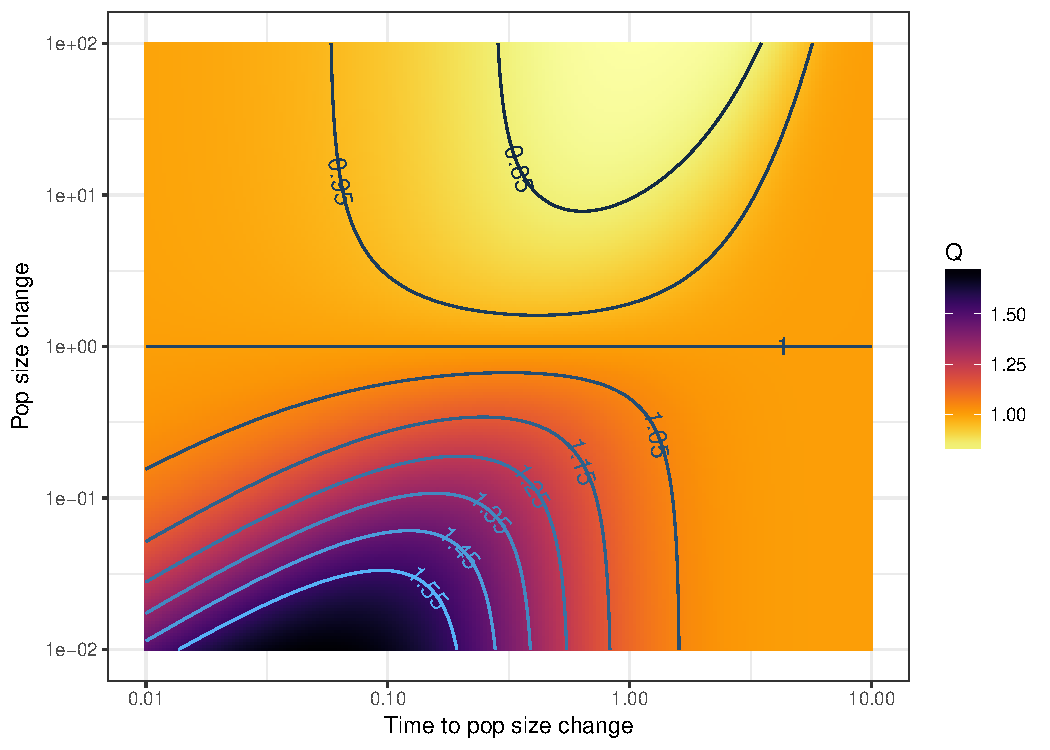
\includegraphics[width=0.9\textwidth]{Q_land.pdf}
  \caption{The scaling factor under different step population size
    changes.}
\end{figure}
Figure \ref{fig:Qland} shows how the expected excess in the fourth population
moment depends on the parameters $b$ and $c$ of the population size change. 
%%% mode: latex
%%% TeX-master: "notes.tex"
%%% End: 
